\documentclass[10pt]{article}


%--------- Packages ----------------

\usepackage{graphicx} % Required for inserting images
\usepackage[a4paper,left=1in,right=1in,top=1in,bottom=1in]{geometry}
\usepackage{newtxtext} % If you need to use Time New Roman
\usepackage{newtxmath} % If you need to use Time New Roman
%\usepackage[style=apa,backend=biber]{biblatex}
\usepackage[british]{babel}
\usepackage{csquotes}
\usepackage{bookmark}
\usepackage{setspace}
\usepackage{fancyhdr}
\usepackage[font=footnotesize,justification=centering]{caption}
\usepackage{hyperref}
\usepackage{float}
\usepackage{setspace}
\usepackage{xcolor}
\usepackage{comment}

%--------- Set Up ------------------
\setstretch{1.0}
\pagestyle{fancy}
\fancypagestyle{plain}{%
  \renewcommand{\headrulewidth}{0pt}%
  \fancyhf{}}
%\addbibresource{references.bib}


% --- title insert (check title.tex for more)----------

\title{A Library for Simulating Thick Origami Kinematics} % TITLE HERE 
\author{ Jacob Pavelka \\ Anvay Pradhan  \\   Noah Zambrano \\} % AUTHOR HERE

%-------- Document -----------------

\begin{document}

%%% Commenting Commands
\newcommand{\Jacob}[1]{{\normalsize{\textbf{({\color{blue} Jacob:\ }#1)}}}}
\newcommand{\Anvay}[1]{{\normalsize{\textbf{({\color{red} Anvay:\ }#1)}}}}
\newcommand{\Noah}[1]{{\normalsize{\textbf{({\color{green} Noah:\ }#1)}}}}

\begin{titlepage}


\newcommand{\HRule}{\rule{\linewidth}{0.5mm}} % Defines a new command for the horizontal lines, change thickness here

% ----- Logo UM ---------

\center

\includegraphics[width=10
cm]{Graphics/logoUM.png}\\[0.1cm]


\textsc{\large NERS 570 project}\\[1cm]

\makeatletter
\rule{\linewidth}{0.2 mm} \\[0.4 cm]
{\huge\bfseries \@title \par} \
\rule{\linewidth}{0.2 mm} \\[1.0 cm]
 \textsc{Nuclear Engineering and Radiological Sciences\\2023}\\[1.5cm] % Name of your program

\begin{minipage}{0.2\textwidth}
\emph{Authors:}\\
\@author 
\end{minipage}
~
\begin{minipage}{0.4\textwidth}
%\begin{flushright} 

% ID HERE

%\emph{Id :} \\
%i0000000\\ i0000000\\ i0000000\\ i0000000
%\end{flushright}
\end{minipage}\\
\vspace{1cm}
\emph{Course Coordinator:}\\
Prof. Brendan Kochunas\\
\vspace{1cm}
\makeatother
{\large \today}\\[2cm] % Date, change the \today to a set date if you want to be precise
\vfill % Fill the rest of the page with whitespace





\end{titlepage}




\fancyhf{}
\setlength{\headheight}{33pt}
\fancyhead[L]{\nouppercase{\leftmark}}
\fancyhead[R]{
\includegraphics[width=0.7cm]{Graphics/UM_SMALL.png}}
\fancyfoot[R]{ \bf\thepage\ \rm }
\fancyfoot[L]{\emph{NERS 570 project} }

\newpage
%\Large{\textbf{Abstract}}
\section*{Abstract}
Kinematic simulations are often the first step in analyzing the motion of a body or set of bodies. In this project, a library was developed that can produce a kinematically admissible motion given a target motion and rigid bodies in the system. This library was created to simulate the kinematics of thick origami. The library was developed according to a waterfall development pattern whereby multiple steps were taken prior to writing code to ensure efficient code architecture. This included creating a formal problem definition consisting of high-level and functional requirements and class and state diagrams.

This project also employed common software development practices. In particular, all code and documentation was handled within GitHub. Here, issues and tasks could be delegated to individual group members to complete the high-level design, low-level design, construction, and testing portions of the code. Further, CMake was used for linking and makefile generation. Object oriented design and version control through Git were utilized throughout. External performant libraries were used for efficient matrix computations. 

The developed library is able to take a JSON file input corresponding to some set of rigid bodies and the desired target velocity and output a visualization showing the folding motion of the bodies. Individual portions of the code were tested and verified before running full example scenarios. The results for two different folding examples are shown with some limitations of the simulations discussed. This library was shown to be able to successfully simulate kinematically admissible motion of input rigid bodies. Additionally, designers of the library gained valuable experience in kinematic simulations and proper software engineering practices. Future work would seek to improve the simulation by simplifying the input file generation, adding more realistic physics, and reducing error through better iteration schemes. 
\newpage
\tableofcontents
\newpage
\newpage
\section{Introduction}
Kinematic simulation is an important tool for many problems. For example, it is used to study the degrees of freedom or range of motion for linkage systems, or to simulate motion for virtual reality training, video games, rapid digital prototyping, and robotics simulation \cite{SiggraphContact22}.
For structural systems, it allows one to study whether or not a system is stable. For example, understanding the kinematic properties of thick origami is important if it were to be used structurally. A kinematic simulation would show which forces would cause the origami to deform without resistance \cite{filipov2015toward}. 
For our project, we wanted to develop a kinematic simulation library for thick, rigid origami so we could become more familiar with kinematic simulation methods and develop performant software that others could use. To test our package, the kinematic folding motions for a cube folded from flat and Miura origami pattern were simulated. The objectives of this project aimed to incorporate the course themes and were defined as follows: 
\begin{itemize}
    \item The library shall be able to simulate the kinematics any convex rigid body that can be sufficiently described by its vertices.
    \item The library shall make use of performant linear algebra libraries.
    \item The library shall make use of Object-Oriented Design.
    \item The library shall make use of design patterns.
    \item The library shall use a CMake based build system.
    \item The library shall use C++ mainly and C if needed.
    \item The library shall incorporate testing.

\end{itemize}


\subsection{Kinematic Simulations}
The kinematics of an origami object can be simulated by first defining the origami's mesh based on predefined nodes, then imposing constraints on those nodes' degrees of freedom based on the defined mesh, and finally, solving for the mesh's kinematically admissible motion based on the constraints \cite{zhu2022review}. 
%
\begin{figure}[H]
    \centering
    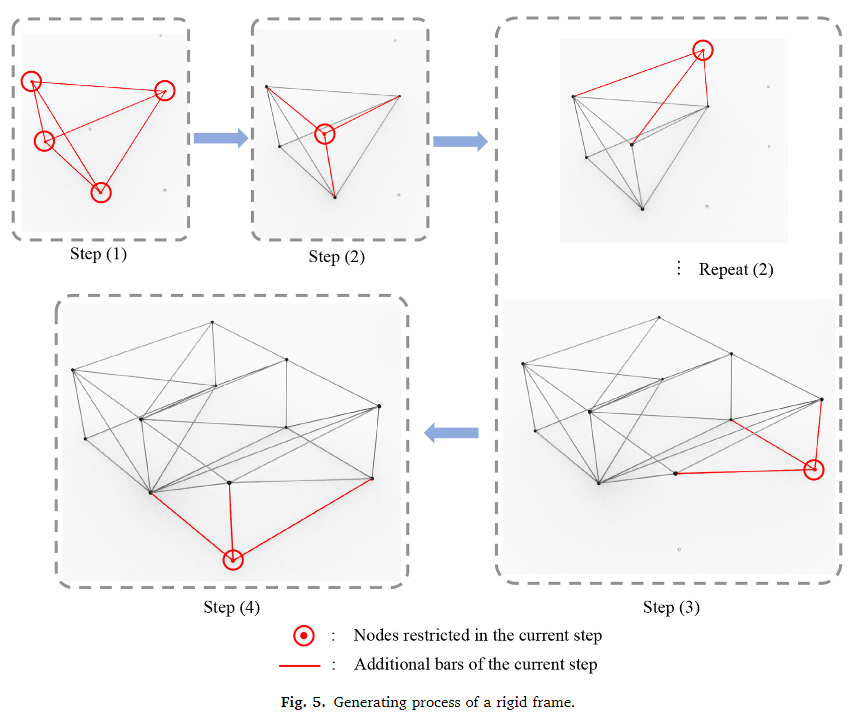
\includegraphics[width=0.6\columnwidth]{Graphics/mesh_gen.png}
    \caption{Procedure for generating a mesh given predefined nodes \cite{zhang2021folding}.}
    \label{fig:mesh_gen}
\end{figure}
%
To simulate the kinematics of an object, it first needed to be represented mathematically, which was done by creating a mesh of the object. There are many methods for creating meshes, but we used the one described in \cite{zhang2021folding} because it creates a mesh of edges and nodes that is automatically stable and minimally rigid.

This algorithm begins with a list of nodes that describe the important features of a convex hull, such as any corners. From here, four nodes are chosen randomly such that they create a tetrahedron, and links are defined between them. Then, another point is chosen randomly and connected to three existing points such that they all form another tetrahedron. Links are created between the three existing nodes and the new node. This process was repeated for all remaining nodes. Figure \ref{fig:mesh_gen} illustrates this. This process created the mesh for one rigid object, but to have objects that could develop complex motion, one or more objects needed to be connected. This was taken care of by grouping objects as bodies.

\subsubsection{Constraints}
Once all points were connected, a connectivity matrix could be formed, and from this, the constraints could be formed. 
The constraint equations of a kinematic system determine what motions are admissible. Constraint equations are determined by conditions such external physics, contact, friction, or geometry. For this library, we focused on purely geometrical constraints, where nodal locations of a rigid body must retain their originally specified distance from each other. If nodes $i$ and $j$ are connected by an edge, then their constraint equation would be
\begin{equation}\label{eq:edge}
    (u_i-u_j) \cdot (u_i-u_j) = l_{ij}^2,
\end{equation}
where $l_{ij}$ is the original distance between nodes $i$ and $j$, and $u_i$ is the coordinate of node $i$. Essentially, this constraint ensures the lengths of the edges remain constant throughout the folding motion.
Rigid bodies were connected along their nodes, where a node might belong to multiple edges. Each constraint defined by the edges was then linearized by taking its derivative with respect to time.
\begin{equation}\label{eq:con-linearized}
\frac{d}{dt}(u_i-u_j) \cdot (u_i-u_j) = \frac{d}{dt}l_{ij}^2.
\end{equation}
Since the body was rigid, its time derivative must be zero,
\begin{equation}\label{eq:con-rigid}
(u_i-u_j) \cdot (\dot u_i-\dot u_j) = 0,
\end{equation}
where Equation \ref{eq:con-rigid} can be decomposed into its cartesian components,
\begin{equation}\label{eq:con-components}
(x_i-x_j) (\dot x_i - \dot x_j)+(y_i-y_j) (\dot y_i - \dot y_j)+(z_i-z_j) (\dot z_i - \dot z_j) =0.
\end{equation}
This constraint was then defined for each pair of nodes connected by an edge, which yielded the system of equations,
\begin{equation}\label{eq:con-system}
C \dot d = 0,
\end{equation}
where $\dot d$ was a vector of velocities for each node's degrees of freedom,
$\dot d = [\dot x_0,\dot y_0,\dot z_0,\dots,\dot z_n]^T$.
Finally, some nodes needed to be constrained relative to the global coordinate system (i.e. boundary conditions). These were called \textit{fixities}. Fixities were implemented into the system of equations by requiring the specified degree of freedom's velocity to be zero and adding the appropriate equations to the constraint matrix.
\begin{equation}\label{eq:con-fixities}
\dot x_i = 0 
\end{equation}

\subsubsection{Admissible Motion}
The constraint matrix encodes all requirements for valid motion. Once the constraint matrix was defined, kinematically admissible velocities could be computed by solving Equation \ref{eq:con-system}. However, $C \in \mathbb{R}^{n \times k}$  where $n < k $, so this system of equations has many solutions. An easier way to find kinematically admissible velocities was to project a target velocity profile onto the null space of the constraint matrix.
\begin{equation}\label{eq:null-space}
\dot d = (I-C^{+}C)\dot d_0
\end{equation}
Where $C^+$ is the pseudo-inverse of $C$ and $\dot d_0$ is the target velocity.
In this way, the admissible velocity closest to the target velocity was chosen. Any numerical integration method may then be used to compute the displacements caused by these velocities. The simplest ODE solving scheme (but most likely to cause errors for long simulations) is the Euler method:
$$d_{i+1}=d_{i}+h\dot d_{i}$$

Where $h$ is the time step. Choosing a time step that is too large leads to larger distortion of the rigid bodies during simulation. Other methods that can be used are Heun's Method or any Runge-Kutta Method. These higher order iteration schemes would reduce the amount of error.



\section{Description of Work Performed}
We defined several tasks in our proposal, and each of these tasks relates to topics learned in class. This section discusses the work performed for the project categorized by the relevant class topic.
\subsection{Waterfall Development Pattern}
One important objective for this project was to employ good software development practices, which meant including all stages of development and employing a development pattern. Using the waterfall development pattern, we first developed high-level ideas about our project, such as defining the problem our library would solve, and ended with working on more concrete tasks, such as defining unit tests for our software. We developed high-level requirements, functional requirements, and class and state diagrams for this project. After the problem definition, requirements, and architecture were defined, Each programmer performed high-level design, low-level design, construction, and testing steps on the tasks they were assigned. 

This work related to the workflows lab, the software engineering lecture where we learned key steps in the software engineering process, including the importance of establishing requirements early and choosing the correct development workflow.
\subsection{GitHub Repository}
After the more abstract stages of the waterfall development pattern were completed, we began to delegate tasks using the issue feature on GitHub. Up to this point, we had already been using GitHub as repository and Git as a version control system for our various diagrams and documents. However, at this point it would also become a place to delegate and collaborate. At the start of the project, each member was assigned three tasks to complete. These tasks were turned into issues, and most issues were turned into branches where the library's development took place. Issues were assigned to people, given tags, and placed on a project for later tracking. We also used the GitHub project to construct a timeline of when certain issues should be completed, and reminders were given to teammates when their tasks were nearing their due date. 

Once each issue was defined, the person assigned to the issue was asked to review it and determine if any other clarification was needed. Apart from that, the assignee could begin to work on that library feature and would eventually merge it into the main branch. 

Finally, once tests started to be written for the library, we implemented continuous integration by running all tests on GitHub and requiring them to pass before a branch can be merged into the main branch.

This work related to the "tools of the trade" lecture and labs 6 and 7, where we learned the importance of version control for stability and collaboration and the usefulness of GitHub for hosting a repository and coordinating group work.
\subsection{Object-Oriented Design}
We employed the object-oriented paradigm for our library using C++. In total, eight classes were used in our library. However, the Structure, Body, Edge, and Node classes were the most relevant classes because they defined the main objects that were used in the simulation. The full list of classes that were used is provided in Table \ref{tab:classes} along with their main purpose.
\begin{table}[H]
\centering
\caption{Okin Library's Classes}
\label{tab:classes}
\def\arraystretch{1.05}
\makebox[\textwidth][c]{
\begin{tabular}{|c|p{100mm}|}
\hline
\textbf{Class}                   & \textbf{Purpose} \\ \hline
Structure & Aggregate all bodies,nodes, and edges and provide an interface to the user for simulation  \\ \hline
Body   & Aggregate nodes and edges and provide a basis for minimal rigidity  \\ \hline
Edges  & define a connection between nodes and all properties related to that connection (distance, etc.)  \\ \hline
Nodes   & Encode the geometry of a structure  \\ \hline
LinAlg   & Perform linear algebra routines needed in the Structure class  \\ \hline
JsonParser   & Acts intermediary between input/output files defined in JSON and the Structure class  \\ \hline
JsonNode   & Provides a basic unit of data in the JsonParser's hierarchical structure  \\ \hline
tVelocity   & Encode the various types of velocities that can be defined by the user so they can be used in the simulation  \\ \hline
\end{tabular}
}
\end{table}

This work related to the "Lifecycle and OOP" lecture where we learned about the different characteristics of objects in OOP, such as encapsulation and inheritance, and how different objects can be related. This work also relates to programming best practices learned in homework 3.
\subsection {Compilation and External Libraries}
This library used CMake to simplify compilation and incorporate mature linear algebra libraries. A description of how this was done is given as well as justification for why we chose to do it this way.
\subsubsection{CMake}
For this library, CMake was used to generate the makefiles and complete all the library linking. CMake was chosen because it is adaptable to various system configurations and makes compilation straightforward for all users. We were also able to specify what kind of compiling options we wanted, such as which libraries to link or which compiler to use. In addition, we also implemented conditional compiling for the external libraries, where if the \texttt{find\_package(...)} command does not automatically find libraries, the code will still compile but with limited linear algebra abilities. 

% Figure \ref{fig:compilation} shows the flow of information in the CMake and Make process. The main workspace contained all the source and header files, which was added to the CMake sub-directories in the CMakeList. From the project workspace, we executed \texttt{cmake -S. -B./build} which then created the build directories which had the same file structure as the main project workspace. This build directory is system-dependent, and is ignored by Git when code is pushed to the repository. From the build file we then went into each source directory and executed the \texttt{make} command which then created the exectutables.

This work relates to several themes in class where we learned about pre-processing, compiling, linking, and installing. Linking external libraries into our library was similar to the PETSc lab, where we had to make sure we were using CMake correctly by ensuring it was able to find all the libraries required. The conditional compiling we used was similar to the examples shown during the ``Elements of Development" lecture. Setting up CMake in our file structure showed our mastery of the learning objectives presented in the ``Tools of the Trade" lecture.
% \begin{figure}[H]
% \centering
% 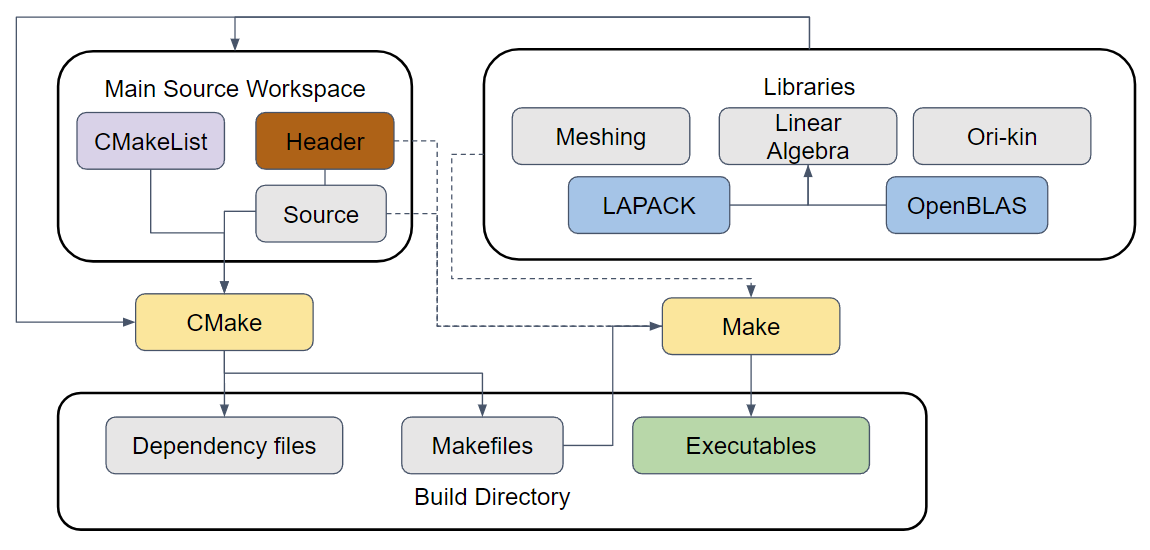
\includegraphics[width=0.8\textwidth]{Graphics/cmake.PNG}
% \caption{CMake compiling flow chart for the ori-kin library}
% \label{fig:compilation}
% \end{figure}
\subsubsection{Linear Algebra Libraries}
Linear algebra was required to determine the kinematically admissible motions of the origami pattern. The required linear algebra functions were described in the introduction. The two main functionalities required were the matrix-matrix multiplication and the pseudo inverse. The pseudo inverse was found using singular value decomposition (SVD),
\begin{equation} \label{eq:svd}
    C=U\Sigma V^T \longrightarrow C^+=U\Sigma ^{-1} V,
\end{equation}
where $C$ was almost always a non-square matrix. From Equation \ref{eq:svd}, it is clear that matrix-matrix multiplication is also required for this step as well as matrix inversion and transposition. While this and the matrix-matrix multiplication can be manually programmed, we decided to use a mature and performant external linear-algebra library. 

This work relates to course topics related to performance and linear algebra routines and libraries. Knowing it would be very difficult to create our own implementation of these algorithms that perform as well as these libraries on all platforms, using open-source linear algebra libraries allowed for efficient computing with minimal cache misses. Any linear algebra routines we implemented would have not used the underlying CPU architecture efficiently and would have resulted in high-bandwidth consuming operation.
\subsection{Visualization}
To provide a way to visualize simulations once they were complete, we extended the JSON parser input class to be able to write results out to a JSON file. Once written to a file, the simulation data could then be read by Python to create visualizations. To do this, we used the Blender visualization software along with the Blender Python module ``bpy". We wrote a Python script to load in all geometry data and combine it with the location history data to make the animations. Specifically, Blender requires an input Object and Mesh to define the visualization. The Object is analogous to a Structure in our C++ library while a Mesh contains all the geometric data, such as vertices, edges, and faces. However, generating a visualization from these two inputs alone generated a single static object. To enable us to view the actual folding motion, each data entry in the JSON file was written to a specific key frame. These key frames could then be played in succession to view the folding motion. From here the animations could be exported to many different video file formats.

This work relates to the scripting module, where we used the bash scripting language to perform similar data manipulation.
\subsection{Testing}
Unit and verification tests were written for our library, where unit tests would verify small components and verification tests would validate that our computations match the background mathematical model. Unit tests were written to verify the instantiation of the Node, Edge, Body, and Structure objects, paying special attention to how many objects were being copied versus passed by reference. Other unit tests verified that an object's properties in memory matched what was specified on the input file. Verification tests were written to verify computations performed in the intermediate stages of the initialization and simulation. For example, a test was written to verify that an angular target velocity specified in the input file was properly converted to a cartesian velocity. Most of these verification tests were constructed based on hand-calculated examples. These tests were incorporated with CMake so that they could be run automatically by us during development and by GitHub for continuous integration purposes.

This work relates to the "Lifecycle and OOP" lecture, the "Verification and Validation" lecture, and Homework 3 where we covered the different types of testing and used CMake to automatically run tests.



\section{Results and Discussion}
We were able to develop a library for simulating the kinematics of a system of rigid bodies. More specifically, we solved our project problem description, that is, we developed a library that could produce a kinematically admissible motion given a target motion and the definition of the rigid bodies in the system. To showcase our library, we developed the two more complex examples from the three originally proposed. These examples were a cube folding and a Miura origami pattern folding. The cube can fold well given five angular velocities related to the five joints that need to fold. The Miura pattern was difficult to fold into its iconic configuration due to the nature of the simulation. Due to how we implemented the library, most of the complexity of performing these simulations is in making the input file.

While the library is always able to simulate an admissible motion, it does not always simulate the motion you would expect from your defined target velocities. This makes the animation ``wiggly" in terms of the cube folding, and makes certain folding motions hard to achieve in terms of the Miura folding. Oftentimes, the target velocity that is specified is a scaled component of the usual basis of a space with a dimension equal to the number of degrees of freedom of your system. This target velocity will most likely not be in the null space of the constraint matrix, so it must be projected to it. When the size of the vectors in the null space becomes large (the degrees of freedom of the structure is large), it is difficult to determine where that vector will project. Sometimes it projects to an admissible velocity that would seem counterintuitive. If multiple target velocities are specified for the same time step, then achieving an admissible velocity that represents the motion desired becomes more feasible, but determining all those target velocities becomes cumbersome. 

The drawback of this library is mostly a feature of the method we chose to select an admissible velocity from all that is possible, which is to project on the null space. Many others are possible, such as using Lagrange multipliers to minimize a Newtonian equilibrium equation.

The rest of this section will be focused on presenting more specific results mirroring the work performed in the previous section, making sure to reflect on lessons learned, the usefulness of the work, and how it could be done better in the future.
\begin{figure}
    \centering
    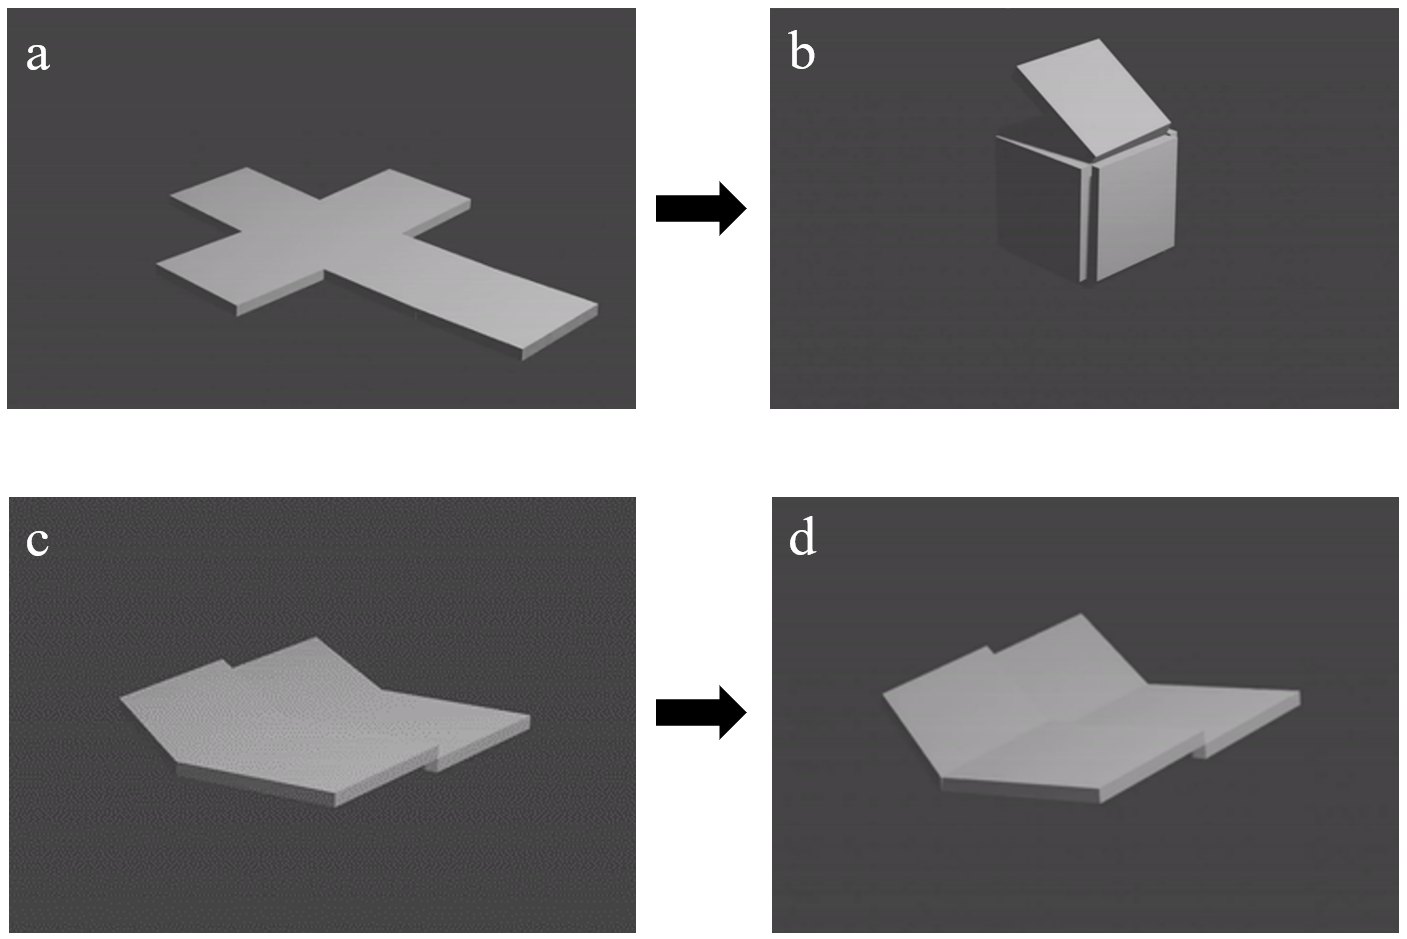
\includegraphics[width=0.9\linewidth]{Graphics/folding_examples.png}
    \caption{Example outputs from ori-kin library. (a) Shows unfolded cube example and (b) shows its folded state. (c) Shows unfolded Miura origami pattern example and (d) shows its partially folded state.}
    \label{fig:folding_examples}
\end{figure}

\begin{comment}
\begin{figure}
    \centering
    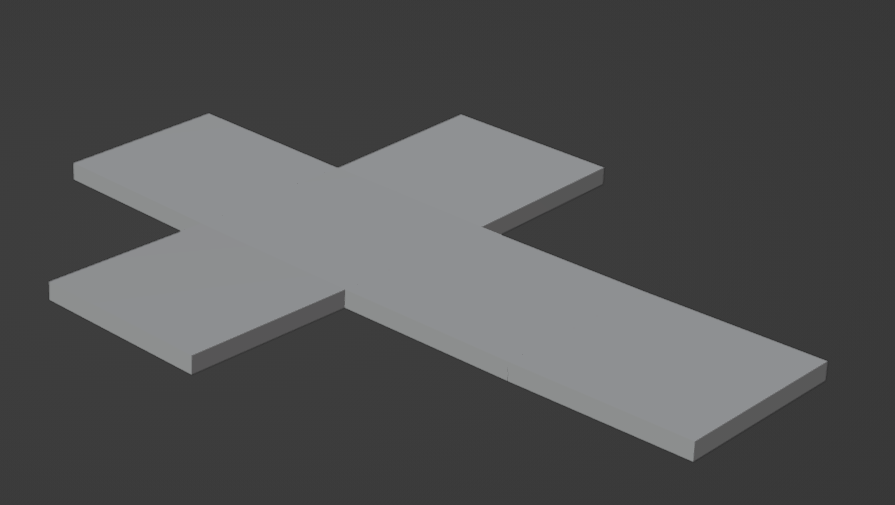
\includegraphics[width=0.5\linewidth]{Graphics/cube_unfold.png}
    \caption{Enter Caption}
    \label{fig:enter-label}
\end{figure}
\begin{figure}
    \centering
    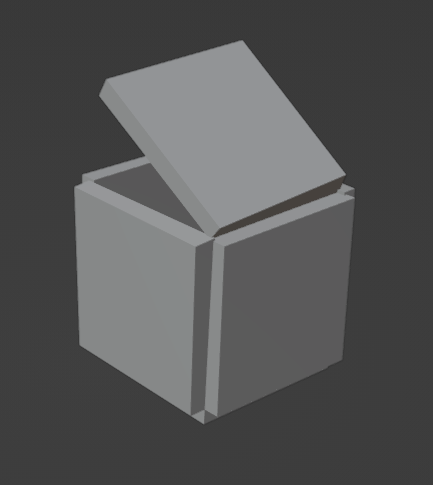
\includegraphics[width=0.5\linewidth]{Graphics/cube_fold.png}
    \caption{Enter Caption}
    \label{fig:enter-label}
\end{figure}
\begin{figure}
    \centering
    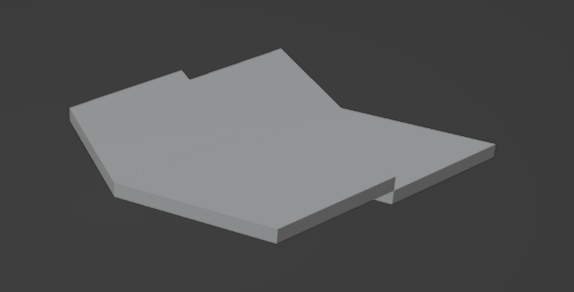
\includegraphics[width=0.5\linewidth]{Graphics/miura.png}
    \caption{Enter Caption}
    \label{fig:enter-label}
\end{figure}
\begin{figure}
    \centering
    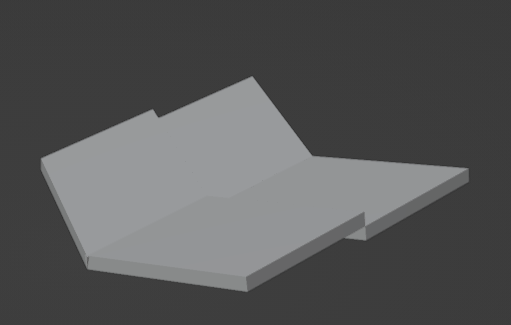
\includegraphics[width=0.5\linewidth]{Graphics/miura_fold.png}
    \caption{Enter Caption}
    \label{fig:enter-label}
\end{figure}
\end{comment}

\subsection{Waterfall Development Pattern}
The problem definition for our project was chosen as:``Develop a library to simulate the motion of constrained rigid bodies based on a given input motion."
We chose our high-level objectives to reflect the goals we had for our project in its proposal. The high-level requirements are the goals stated in the introduction.
% \begin{itemize}
%    \item The library shall be able to simulate the kinematics any convex rigid body that can be sufficiently described by its vertices.
%     \item The library shall make use of performant linear algebra libraries
%     \item The library shall make use of Object-Oriented Design
%     \item The library shall make use of design patterns
%     \item The library shall be extensible
%     \item The library shall use a CMake based build system
%     \item The library shall use C++ mainly and C if needed
% \end{itemize}

The functional requirements were developed to reflect the tasks defined in the proposal and any other requirements we realized after the fact. These functional requirements are as follows:

\begin{itemize}
    \item The library shall generate a complete mesh of a system of rigid bodies given an input file of each rigid body's relevant vertices.
    \item The library shall define a constraint matrix for a defined rigid body based only on the defined mesh and current position.
    \item The library shall compute a constrained set of velocities given a general velocity of interest and update the mesh positions based on a specified integration scheme.
    \item The library shall support calculations in double-precision arithmetic.
    \item The library shall provide a method for visualizing the constrained motion.
\end{itemize}

The library architecture, represented by our state and class diagrams, implemented a design we thought would be sufficient for our library. Ideally, we planned to only proceed through this process once since the library would be relatively simple. However, once we began the high and low-level design of our library, we quickly realized small modifications to the architecture would simplify the library's development. Because of this, we had to revert to the earlier architecture development steps to make these simplifications. In this sense, the final development pattern that was employed was closer to an iterative or agile one. This may have led to more efficiency overall because we did not need to spend excessive time in earlier development steps making sure we caught every detail, considering that most important details can't be seen until later steps. The final state and class diagrams are shown in Figures~\ref{fig:class}-\ref{fig:state}

\begin{figure} [H]
\centering
%\begin{minipage}{.5\textwidth}
  \centering
  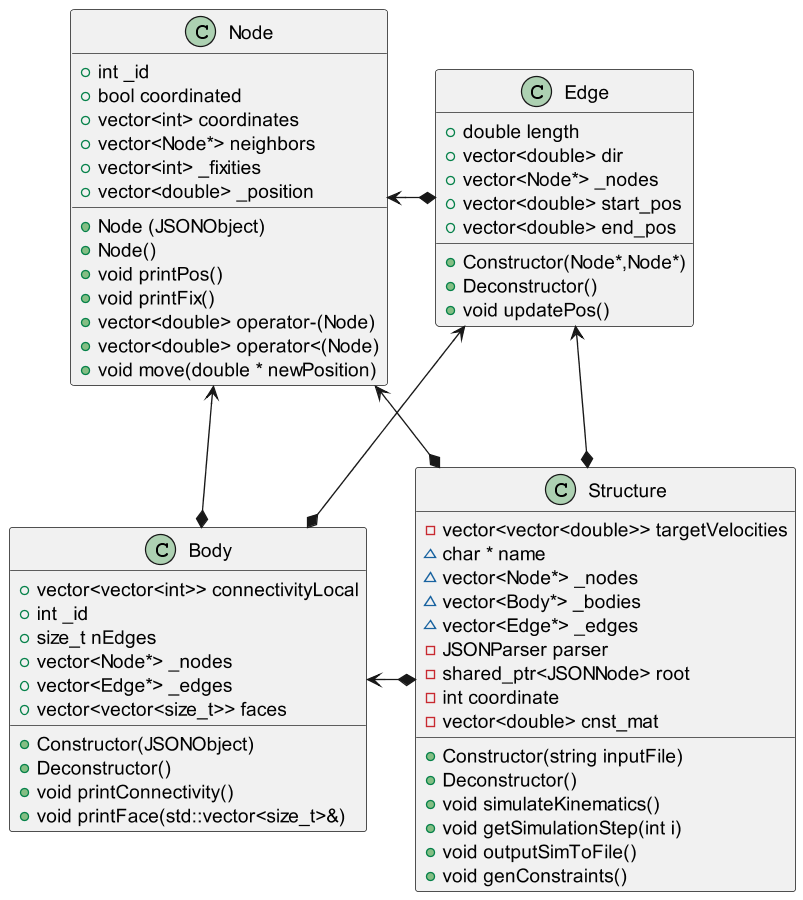
\includegraphics[width=0.7\linewidth]{Graphics/classNew.png}
  \captionof{figure}{UML class diagram of the most relevant classes in the ori-kin library}
  \label{fig:class}
  \end{figure}
%\end{minipage}%
%\begin{minipage}{.5\textwidth}
\begin{figure} [H]
  \centering
  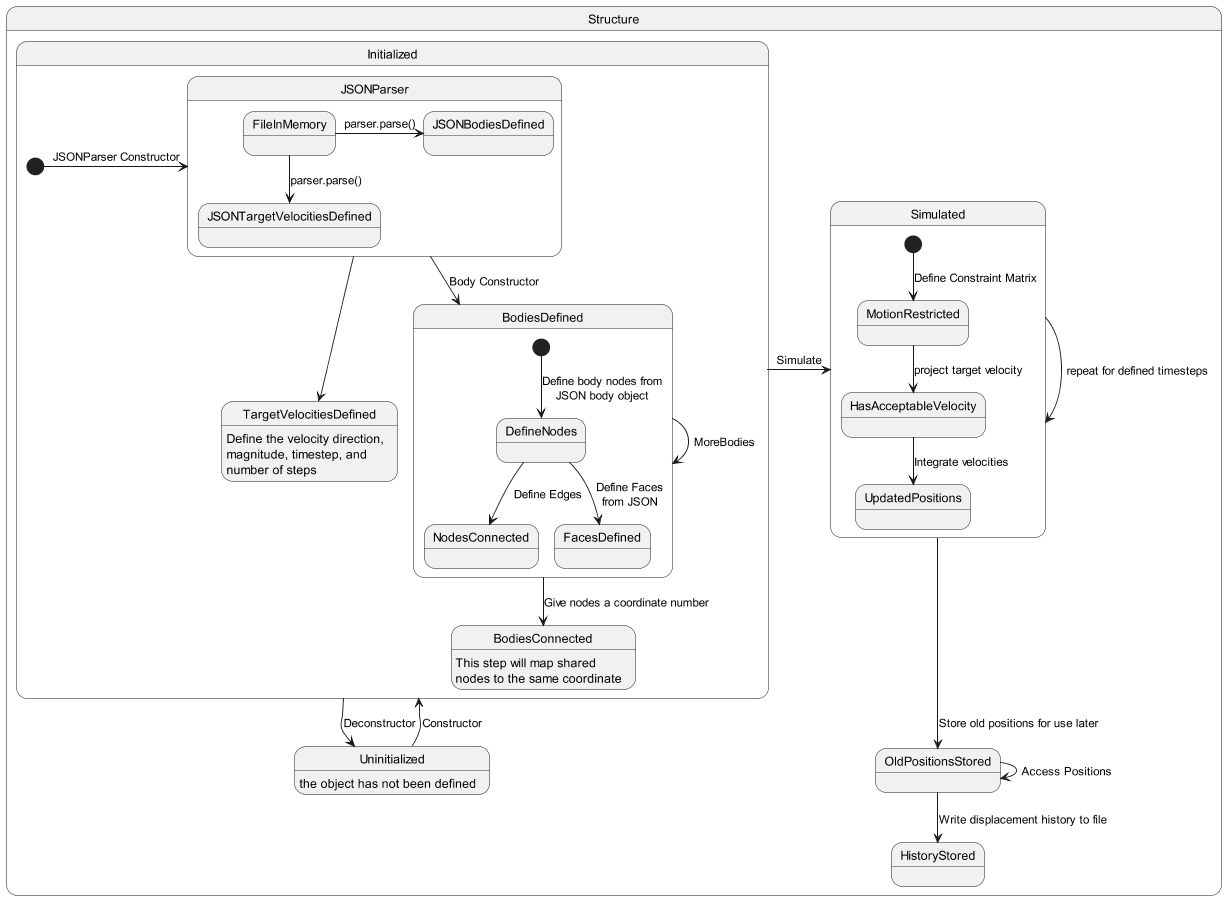
\includegraphics[width=0.7\linewidth]{Graphics/stateNew.png}
  \captionof{figure}{UML state diagram of a user's typical interaction with the library}
  \label{fig:state}
%\end{minipage}
\end{figure}
While the high-level requirements, functional requirements, and architecture were not critical to the library, taking the time to perform these non-essential earlier development tasks allowed for later essential tasks (high-level design, low-level design, etc.) to be completed more efficiently because we had a clear idea of how each component needed to interact with other components. Additionally, thinking through these earlier tasks likely reduced the amount of rework that would have been needed for this library.

\subsection{GitHub Repository}
Overall, our GitHub repository became more than a place to delegate work and combine our code. It became a place to work together and help solve each other's problems. The GitHub issues allowed for more than just task delegation. They also allowed us to completely describe and understand the task at hand before any code was written. Using GitHub projects, we could keep track of issues and manage their states more easily, allowing us to keep the project relatively on track. 

However, the management features of GitHub were mostly overkill, such as assigning labels, requiring reviews on pull requests, and putting issues in different bins. This is because we were a relatively small team with a relatively simple project, but using these features did give insight into how they can be useful on larger, ongoing projects that invite open-source collaboration and have issues submitted by people external to the core team. Besides using the issues to define the tasks well before we started working on them, most of the GitHub management features were done purely for housekeeping and provided no new information. The continuous integration features had a similar significance to the management features because we would have lengthy offline discussions about a branch before it was merged into the main one. In a larger, more distributed project, these features would have been critical.

The shared repository feature of GitHub was the most important for us. Using this feature, we could easily discuss problems we were having in our development by analyzing the changes made on someone's last commit. Then, we could propose our own changes based on a solution derived from our own expertise. For example, at one point, there was a bug in the branch responsible for developing the simulation method of the structure class. Jacob suspected there might have been an issue with the pseudo-inverse function, but was not as familiar with it as Noah, who implemented it. After committing his changes, Jacob asked Noah to review it to see if there is an issue. The issue was found and fixed quickly by Noah.
\subsection{Object-Oriented Design}
Using Object-Oriented Programming structures allowed us to combine data and functionality. This made developing the library more efficient because the data that was needed for an operation was easy to access. For example, during initialization, all the geometric and connectivity data for nodes, edges, and bodes are attached to their respective objects, and then their pointers are stored in a list as an attribute of the structure. This greatly simplifies the structure's generate constraint method. Instead of passing all the edges and nodes into the function by reference, they are automatically in the scope of the method and can be called directly. Furthermore, the nodes' and edges' attributes can be easily accessed too.
\begin{verbatim}
void Structure::genConstraints(){
...
full_cnst_mat[i][j] = _edges[i]->start_pos[0]-_edges[i]->end_pos[0];
...
}
\end{verbatim}

Special methods could also be implemented for each object to simplify common operations on the object's attributes. For example, the difference in node positions often needed to be computed, so instead of manually iterating through each position for every occurrence of this operation, we overloaded the subtraction operator on the node class so that node objects could be subtracted and a vector representing their difference could be returned
\begin{verbatim}
vector<double> Node::operator-(Node input){
    vector<double>res{0.0,0.0,0.0};
    for (int i=0;i<3;i++){
        res[i]=_position[i]-input._position[i];
    }
    return res;

}
\end{verbatim}

One of the biggest features of object-oriented programming is encapsulation, however, due to limited development time, we had to make most of the variables public for testing purposes. The alternative to this would be to make specific accessors for each variable we wanted to test. Not implementing this feature of object-oriented programming will make the software more susceptible to misuse by users and result in errors that are not obvious or caught by the program. 
\subsection{Compilation and External Libraries}
Using CMake made our library more portable, easier to recompile, and easier to integrate external libraries. 
We chose to use LAPACK and OpenBLAS external libraries \cite{anderson1999lapack} to perform the linear algebra operations since they are open source libraries with more mature algorithms than anything we could develop in the given time frame. The LAPACKE and cBLAS wrappers were used for this work. LAPACKE required input matrices to be passed as column-major or row-major arrays. We chose to pass them as column-major arrays which then set the format requirement for the rest of the library. Linear-algebra functions were then written in C++ that call the \texttt{cblas\_dgemm(...)} and \texttt{LAPACKE\_dgesdd(...)} routines. Each function took in column-major vectors rather than arrays to avoid memory leaks and converted them within the function. A pseudo inverse function did not exist in LAPACKE, so we wrote the function ourselves by calling \texttt{LAPACKE\_dgesdd(...)} for the decomposition and performed respective matrix multiplication with cBLAS. Figure \ref{fig:compilation} shows the flow of information in the CMake and Make process. The main workspace contained all the source and header files, which was added to the CMake sub-directories in the CMakeList. From the project workspace, we executed \texttt{cmake -S. -B./build} which then created the build directories which had the same file structure as the main project workspace. This build directory is system-dependent, and is ignored by Git when code is pushed to the repository. From the build file we then went into each source directory and executed the \texttt{make} command which then created the executables.
\begin{figure}[H]
\centering
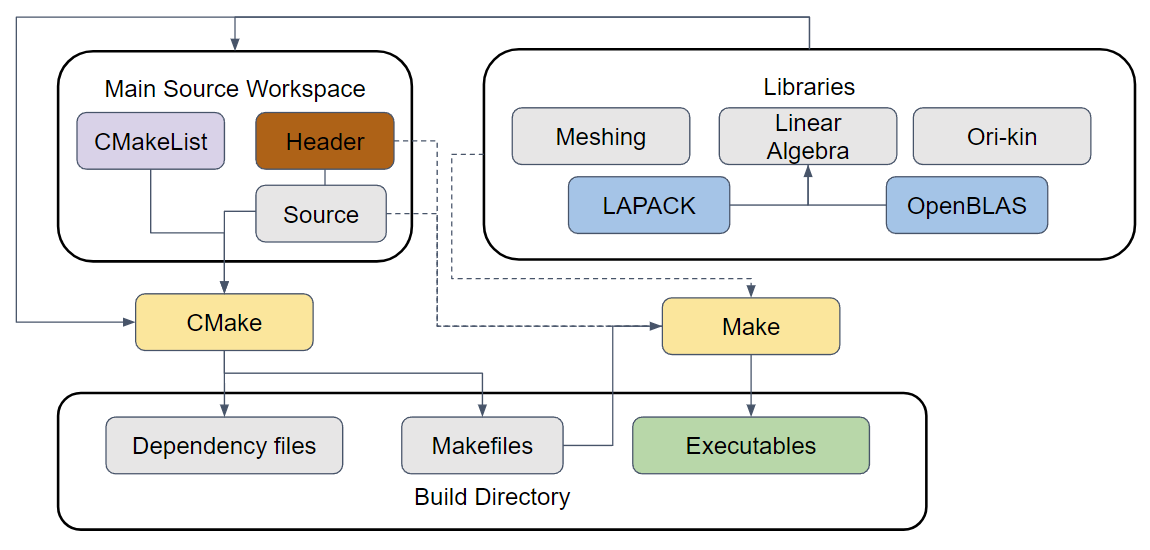
\includegraphics[width=0.8\textwidth]{Graphics/cmake.PNG}
\caption{CMake compiling flow chart for the ori-kin library}
\label{fig:compilation}
\end{figure}
\subsection{Visualization}
As seen in Figure \ref{fig:folding_examples}, we were successfully able to visualize our simulations using the Python scripting language and the Blender executable. This part of our library is important because it is the main medium of interpreting the simulation results. While the script is capable of producing animations, It is much less accessible than our library. The visualization script has static file paths to the output JSON file and output video file, it needs to have a Python version 3.10 library installed with the bpy module, and it must be called explicitly after a simulation to produce an animation. Ideally, these are all issues that could be resolved during the project configuration using CMake, but we did not reach this point in our project. For another user to make an animation with our library, they will need to understand the background processes well, which is bad programming philosophy and does not follow the key ideas of abstraction.
\subsection{Testing}
Testing is a critical step in software design and development. It enables us to find issues quickly and also helps benchmark the code so that when new functionalities are implemented, we can go back to the prior tests and ensure every component is working adequately. It is for this reason that testing cases are implemented with the library. This work details the unit and verification testing of the ori-kin library. We chose to put more emphasis on unit testing so that it would be easier to find small issues that novice programmers (like ourselves) make. 
\subsubsection{Unit Tests}
Unit tests were designed to catch small errors in the routines used throughout the library. These tests were designed to check if a function works in isolation, and therefore does not verify that it would work concurrently with other functions. The five main categories for the unit tests are the parser, meshing, constraint, simulation, and linear algebra tests.
The unit tests for the latter categories consisted of the following tests listed in Tables \ref{tab:meshing_ut}-\ref{tab:linalg_ut}. In the tables, each of their intended checks are described. These tests helped us out greatly, as we found several bugs/errors in all categories. For example, the linear algebra test found an error in linking the LAPACKE library that was not caught in the compilation, the constraints test resolved a bug where the fixities were being assigned but the constraint matrix was not properly sized so it was unable to incorporate the fixities, and so forth. Many unit tests require that geometry is generated from the meshing algorithm. The test mesh used was a simple unit cube. With this simple geometry, we are able to manually verify what the expected output of each function should be.
\subsubsection{Verification Tests}
The verification tests are done to check that the functions work together in a main program that uses multiple functions. This catches errors that unit tests are not able to catch, such as improper variable deallocation, memory leakage, and other hosts of problems. Several sets of verification were implemented in a verification test executable. These tests used a simple cube mesh. The overall projection step using the linear algebra, ODE, and accessor functions was tested by manually computing the expected matrices along each step of the multi-function process and comparing the results with assert statements. This was a major component of the \texttt{Structure.simulate()} function which runs the actual simulation and relies on many other classes and functions. Next, the deallocation features in the linear algebra were also tested, where multiple subsequent uses of the linear algebra functions were compared against a known solution. These tests helped find several memory leaks and deallocation issues. For example originally we passed standard arrays into the linear algebra functions, but when used sequentially, gave errors as some arrays had random values after it was used once in a function. This was resolved by converting storage to vectors and led to discoveries of bugs where we forgot to delete unused memory. Finally the last verification was to ensure the edge lengths remained roughly constant. A rigid treatment means that their change in length should be zero, but it is known that the first-order Euler solver introduces error when solving the ODE, so we expect an error that scales with the number of iterations, but plateaus and remains nearly constant once the kinematics are no longer in motion. Results for this error are shown in Figure \ref{fig:euler-error}, where the expected trend is shown. Finally, proof of all tests passing in GitHub checking is shown in Figure \ref{fig:test-pass}.

\begin{table}[H]
\centering
\caption{Meshing Unit Tests}
\label{tab:meshing_ut}
\def\arraystretch{1.05}
\makebox[\textwidth][c]{
\begin{tabular}{|c|c|}
\hline
\textbf{Test name}                   & \textbf{Purpose} \\ \hline
nodeOrder & ensures node ordering follows expected convention  \\ \hline
allHere   & ensures the right number of bodies and nodes are created  \\ \hline
nodeInit   & checks if nodes positions are correct and if fixites are created  \\ \hline
nodeSub   & checks that distance between nodes is correct  \\ \hline
nodeComp   & checks if node comparsion is valid both ways  \\ \hline
edgeInit   & ensures edge lengths are created correctly  \\ \hline
edgeUpdate   & checks if direction, length, and psoition are correctly updated   \\ \hline
bodyInit   & ensures that faces are correctly created \\ \hline
allCoordinated   &  tests each node to see if coordinated \\ \hline
jointDefined   & ensures node joints are the same value  \\ \hline
\end{tabular}
}
\end{table}

\begin{table}[H]
\centering
\caption{JSON Parser Unit Tests}
\label{tab:parse_ut}
\def\arraystretch{1.05}
\makebox[\textwidth][c]{
\begin{tabular}{|c|c|}
\hline
\textbf{Test name}                   & \textbf{Purpose} \\ \hline
stringParser & checks if strings are correctly read  \\ \hline
listParser & checks if correct string lengths are obtained \\ \hline
nestObjParse & checks if objects are correctly accessed in nest\\ \hline
nestNumPars & checks if object numbers are correctly accessed in nest\\ \hline
trueParse & ensures a true bool value is correctly parsed\\ \hline
falseParse & ensures a false bool value is correctly parsed\\ \hline
multiNestParse & checks if a double nested object is correctly accessed \\ \hline
printJson & checks it parsed output matches read-in file\\ \hline
\end{tabular}
}
\end{table}

\begin{table}[H]
\centering
\caption{Kinematic Simulation/Constraints Tests}
\label{tab:kinsim-con_ut}
\def\arraystretch{1}
\makebox[\textwidth][c]{
\begin{tabular}{|c|c|}
\hline
\textbf{Test name}                   & \textbf{Purpose} \\ \hline
checkCols & ensures that the correct number of rows is created in constraint matrix for test mesh  \\ \hline
checkRow   & checks if the one the the rows is correctly populated based on node coordinates  \\ \hline
projection & checks to see if math for projection onto null-space is correct  \\ \hline
velocityVectorInit & ensures velocity type and values and time stepsize are correctly initalized \\ \hline
normalizeTest & check if normalization is correct  \\ \hline
projectTest & checks to see if projection of two vectors is correct \\ \hline
updateAngle & checks if angle change gives correct velocity change  \\ \hline
strucutreVelAccess & checks functionality of velocity accessor  \\ \hline
\end{tabular}
}
\end{table}

\begin{table}[H]
\centering
\caption{Linear Algebra Unit Tests}
\label{tab:linalg_ut}
\def\arraystretch{1.05}
\makebox[\textwidth][c]{
\begin{tabular}{|c|c|}
\hline
\textbf{Test name}                   & \textbf{Purpose} \\ \hline
pseudoInv & check if pseudo inverse is correct for non-trivial tall-rectangular matrix  \\ \hline
pseudoInvNGrM   & check if pseudo inverse is correct for non-trivial long-rectangular matrix  \\ \hline
matMult  & checks if matrix-matrix multiplication of non-trivial non-square matrix is correct  \\ \hline
matVec   & checks if matrix-vector multiplication of non-trivial matrix is correct  \\ \hline
\end{tabular}
}
\end{table}

\begin{figure}
\centering
\begin{minipage}{.5\textwidth}
  \centering
  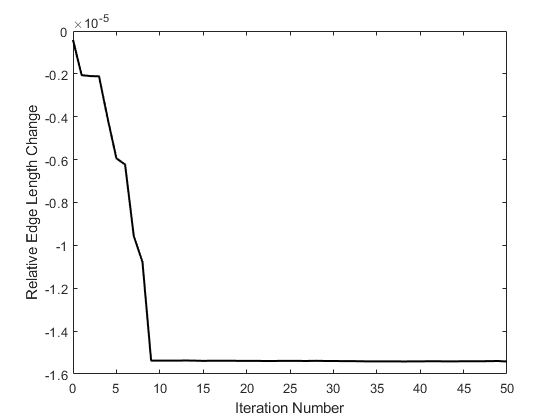
\includegraphics[width=1\linewidth]{Graphics/euler-error.png}
  \captionof{figure}{Change in edge length with respect to number of iterations for a step size of 0.01}
  \label{fig:euler-error}
\end{minipage}%
\begin{minipage}{.5\textwidth}
  \centering
  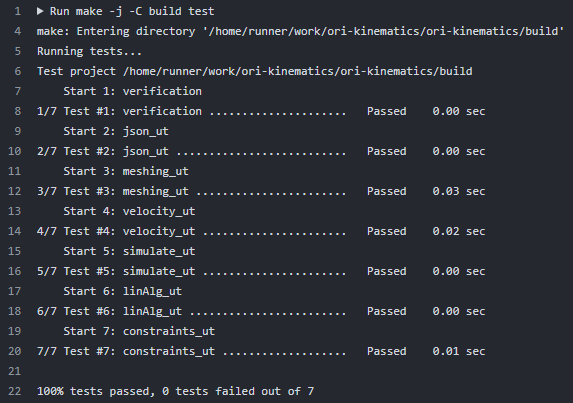
\includegraphics[width=1\linewidth]{Graphics/test-pass.PNG}
  \captionof{figure}{Output of passed tests in GitHub}
  \label{fig:test-pass}
\end{minipage}
\end{figure}
\newpage
\section{Conclusion}
On the surface level, we made a library to perform kinematic simulations. However, the real goal we were trying to achieve was to practice making software close to the level that is done by professionals in scientific computing so that one day, we may make our own scientific computing software that is used by others in the industry. In this way, we believe we met our objective. However the following sections will go into detail on the specific objectives listed in the introduction, as well as things we learned and possible future improvements.
\subsection{Objectives}
Recalling the core objectives, we can discuss whether it was met or not
\begin{itemize}
    \item The library shall be able to simulate the kinematics any convex rigid body that can be sufficiently described by its vertices. \textbf{Almost}. As seen in Miura fold example, we were not able to get the expected motion, but we did however get the cube to work.
    \item The library shall make use of performant linear algebra libraries. \textbf{Mostly}. LAPACK and OpenBLAS were successfully implemented, although it would have been nice to add more performant libraries like PETSC.
    \item The library shall make use of Object-Oriented Design. \textbf{Yes}. The code makes strong use of OOP and all the relevant concepts like abstraction, classes, private/public members, etc. This allowed the code to be quite modular.
    \item The library shall make use of design patterns. \textbf{Yes}. The waterfall design pattern was employ and helped drive the code design.
    \item The library shall use a CMake based build system. \textbf{Yes}. CMake was successfully used and worked wonderfully with the code, making compilation on various environments very easy.
    \item The library shall use C++ mainly and C if needed. \textbf{Yes}. Almost all the code was in C++. We also implemented scripting languages which was a bonus.
    \item The library shall incorporate testing. \textbf{Yes}. Many different unit tests were incorporated and helped us find issues quickly. Verification tests also helped us find unexpected problems, although we could have had more verification tests but ran short on time.

\end{itemize}
\subsection{What was Learned and Value of Work}
A significant amount of learning came along with this project. Learning about C++ and OOP was an invaluable lesson, getting hands-on work and creating our own classes really helped us understand the benefits of OOP and the syntax of C++. Of course, we also learned a lot about kinematic simulations and the math behind it. Going through the weeds and figuring out how to program everything really strengthen our understanding of the numerical methods and linear algebra used to compute the admissible motions. A lot was learned about compilation and linking as well. Having to make the CMake files helped us understand how compilation works on Great Lakes and other environments, as well as the building process and required file structures. The testing also proved to be extremely valuable in debugging code \textit{before} we tried to run cases. It was surprising how many issues it caught beforehand. Finally, we learned a lot about working as a team and using GitHub for code management. Using GitHub helped us learn to to state our problems and update our work. The process of creating pull requests or merging code or creating branches was very valuable and will help us work with others in the future. We come out of this project with a good base for a more powerful origami kinematics library which is valuable to the members whose area of research is origami kinematics. However, what was the most valuable was the lessons learned and experienced gained developing this code and using different tools and methods of the scientific computing field.
\subsection{Areas of Future Work}
There are several areas of improvement for future work. The clearest direction is to implement more complicated origami, like the waterbomb pattern. As mentioned before, the biggest hurdle in this is creating the JSON file. More work should also be done to correct any potential mistakes and get the Miura pattern to work before going to more complicated problems, however. Another problem is to include more realsitic physics into the library. We can incorporate external forces that give preference to certain motions, or add friction and contact restraints. We can also do non-rigid bodies as a more complicated problem. We can also implement more powerful libraries, like PETSC. PETSC can be used to implement higher-order schemes like Runge-Kutta for solving the ODE. This would reduce the error between time steps and obtain a more realistic solution.


%\section{Appendix}


\bibliographystyle{plain}
\bibliography{refs}
\end{document}
